\section{From Neurons to Networks}
\begin{frame}{From Neurons to Layers}
    We don't just use one neuron. We stack them in parallel to form a \textbf{Layer}.

    \centering
            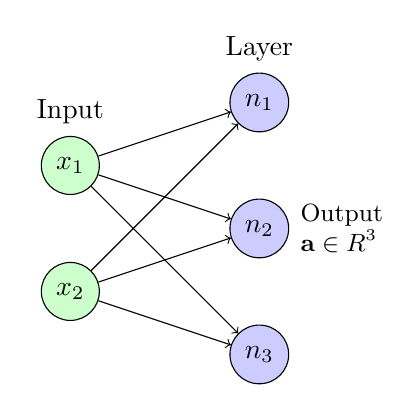
\begin{tikzpicture}[scale=0.8]
                % Input
                \node[draw, circle, fill=green!20] (x1) at (0, 1) {$x_1$};
                \node[draw, circle, fill=green!20] (x2) at (0, -1) {$x_2$};
                \node[above] at (0, 1.5) {Input};
                
                % Layer (3 Neurons)
                \node[draw, circle, fill=blue!20] (n1) at (3, 2) {$n_1$};
                \node[draw, circle, fill=blue!20] (n2) at (3, 0) {$n_2$};
                \node[draw, circle, fill=blue!20] (n3) at (3, -2) {$n_3$};
                \node[above] at (3, 2.5) {Layer};
                
                % Connections (Dense)
                \draw[->] (x1) -- (n1); \draw[->] (x1) -- (n2); \draw[->] (x1) -- (n3);
                \draw[->] (x2) -- (n1); \draw[->] (x2) -- (n2); \draw[->] (x2) -- (n3);
                
                \node[right, font=\small, align=left] at (3.5, 0) {Output \\ $\mathbf{a} \in \mathbb{R}^3$};
            \end{tikzpicture}
    
    % \vspace{1.5em}
    
\end{frame}

\begin{frame}{From Neurons to Layers}
    \textbf{How do we decide the number of neurons?}
    
    \vspace{1em}
    \begin{itemize}
        \setlength\itemsep{1.5em}
        \item \textbf{The Input Layer:}
        If our data has $k$ features (e.g., Age, Salary, Debt), the input layer must have $k$ neurons.
        
        \item \textbf{The Output Layer:}
        If we are doing multiclass classification (e.g., Cat, Dog, Bird), the output layer must have $k$ neurons (one score per class).
        
        \item \textbf{Hidden Layers:}
        This is a design choice (Hyperparameter). More neurons = captures more complex patterns.
    \end{itemize}
\end{frame}

\begin{frame}{Network Shapes for Different Tasks}
    \centering
    \small
    \begin{tabular}{l l l l}
        \toprule
        Task 
        & Input 
        & Output of NN 
        & Typical loss \\
        \midrule
        Single output regression 
        & \(x \in \mathbb{R}^k\) 
        & \(\hat{y} \in \mathbb{R}\) 
        & Mean squared error \\
        Multi output regression 
        & \(x \in \mathbb{R}^k\) 
        & \(\hat{y} \in \mathbb{R}^m\) 
        & MSE over all outputs \\
        Binary classification 
        & \(x \in \mathbb{R}^k\) 
        & \(\hat{p} \in (0, 1)\) 
        & Binary cross entropy \\
        Multiclass classification 
        & \(x \in \mathbb{R}^k\) 
        & \(\hat{p} \in \mathbb{R}^C\) softmax 
        & Cross entropy \\
        \bottomrule
    \end{tabular}
\end{frame}

% --- SLIDE 9B: The Math (Matrix View) ---
\begin{frame}{The Math: Vectorization}
    Since a layer is just a collection of neurons running in parallel, we can mathematically represent it using \textbf{Linear Algebra}.
    
    \vspace{1em}
    \begin{columns}[c]
        \begin{column}{1.0\textwidth}
            \begin{itemize}
                \item \textbf{Single Neuron:} 
                $$z = \mathbf{w}^\top \mathbf{x} + b$$
                (Weights are a vector $\mathbf{w}$)
                \vspace{1em}
                \item \textbf{Full Layer:} 
                $$\mathbf{Z} = \mathbf{W} \mathbf{x} + \mathbf{b}$$
                (Weights are a \textbf{Matrix} $\mathbf{W}$)
            \end{itemize}
            
            \vspace{1.5em}
            \small
            \textit{Every row in matrix $\mathbf{W}$ represents one specific neuron's weights.}
        \end{column}
        
        % \begin{column}{0.45\textwidth}
            
        % \end{column}
    \end{columns}
\end{frame}

% --- SLIDE 10: Why Depth? (FIXED IMAGE LAYOUT) ---
\begin{frame}{From Layer to Layers (Going Deep)}

    \textbf{In theory:} One layer is enough to fit anything. \\
    \textbf{In practice:} Deeper networks are much more powerful and efficient.
    
    \vspace{0.5em}
    \begin{itemize}
        \item They learn \textbf{hierarchical features}: \\
        \small (Pixel $\to$ Edge $\to$ Shape $\to$ Face).
    \end{itemize}

    \vspace{0.5em}
    \centering
    % Image now at the bottom, full width
    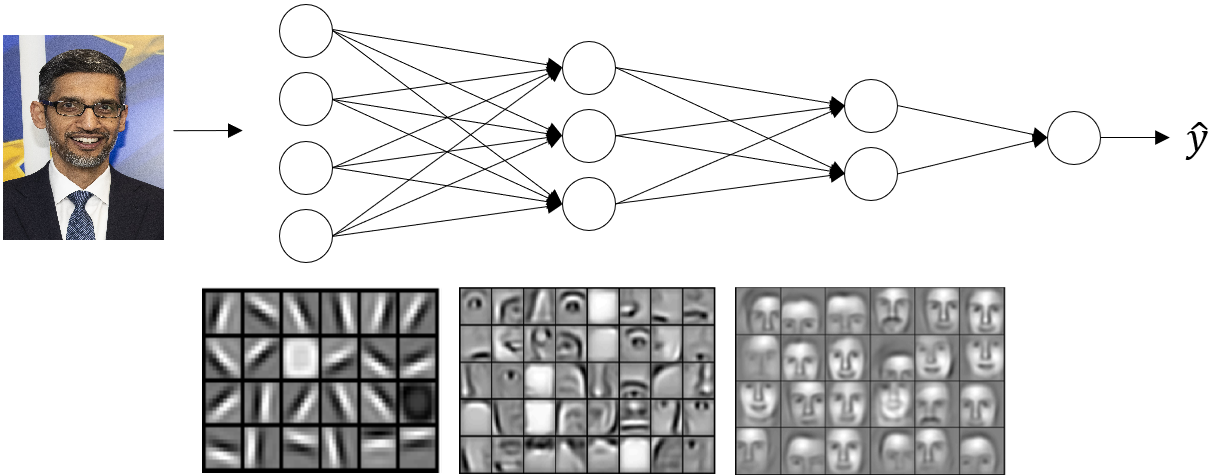
\includegraphics[width=0.95\linewidth, height=0.45\textheight, keepaspectratio]{images/nn_exampe_google_guy.png}
\end{frame}

% --- SLIDE 9: RECURSIVE DEFINITION (End-to-End) ---
\begin{frame}{Putting it Together: The Neural Network}
    A Neural Network is just a \textbf{recursive chain} of these layers. 
    The output of one layer becomes the input of the next.
    
    \vspace{1em}
    \centering
    % Flow Diagram
    \begin{tikzpicture}[node distance=1.5cm, auto, thick, >=latex]
        \node[draw, fill=green!10] (input) {Input $x$};
        \node[draw, right=of input, fill=blue!10] (h1) {Layer 1};
        \node[draw, right=of h1, fill=blue!10] (h2) {Layer 2};
        \node[draw, right=of h2, fill=red!10] (out) {Pred $\hat{y}$};
        
        \draw[->] (input) -- (h1);
        \draw[->] (h1) -- (h2);
        \draw[->] (h2) -- (out);
    \end{tikzpicture}
    
    \vspace{1.5em}
    \raggedright
    \textbf{Mathematically (The Recursive Formula):}
    
    \begin{enumerate}
        \item \textbf{Input:} $h^{(0)} = x$
        \item \textbf{Hidden 1:} $h^{(1)} = \sigma(W_1 h^{(0)} + b_1)$
        \item \textbf{Hidden 2:} $h^{(2)} = \sigma(W_2 h^{(1)} + b_2)$
        \item \textbf{Output:} $\hat{y} = \text{Softmax}(W_3 h^{(2)} + b_3)$
    \end{enumerate}
    
    \vspace{0.5em}
    \small \textit{Data flows from left to right, getting transformed at every step.}
\end{frame}


% --- SLIDE 12: The Training Loop ---
\begin{frame}{Neural Networks as Part of a Learning System}
    \begin{tikzpicture}[
        node distance=2.0cm,
        auto,
        thick,
        block/.style={
            rectangle, 
            draw, 
            rounded corners=5pt,
            text width=2.4cm, 
            text centered, 
            minimum height=1.1cm,
            font=\small\bfseries,
            line width=1.1pt
        },
        line/.style={draw, -{Latex[length=2.3mm]}, line width=1.1pt}
    ]
        % Nodes
        \node [block, fill=gray!20] (data) {Data\\$(x, y)$};
        \node [block, fill=blue!20, right=1.3cm of data] (model) {Neural Network\\$\hat{y} = f_\theta(x)$};
        \node [block, fill=red!20, right=1.9cm of model] (loss) {Loss Function\\$J(\theta)$};
        \node [block, fill=green!20, below=1.0cm of model] (opt) {Optimizer};
        
        % Flows
        \path [line, blue!70] (data) -- node [below, black] {\scriptsize Input $x$} (model);
        \path [line, gray!70] (data.north) to[bend left=15] node [above, black, pos=0.5] {\scriptsize True $y$} (loss.north);
        \path [line, red!70] (model) -- node [below, black] {\scriptsize Predictions $\hat{y}$} (loss);
        \path [line, orange!70] (loss.south) to[bend left=20] node [left, black, pos=0.3] {\scriptsize Compute $\nabla J$} (opt.east);
        \path [line, green!70] (opt) -- node [left, black] {\scriptsize Update $\theta$} (model);
    \end{tikzpicture}

\end{frame}

% In preamble:
% \usepackage{tikz}
% \usetikzlibrary{positioning,calc,arrows.meta}

% --- SLIDE 9: RECURSIVE DEFINITION (End-to-End) ---
